\chapter{核函数和非线性支持向量机}

\section{核技巧}

\subsection*{非线性分类问题}

非线性分类问题无法通过线性模型分类,如下图所示,正例点和负例点混杂在一起。

\begin{figure}[H]
    \centering
    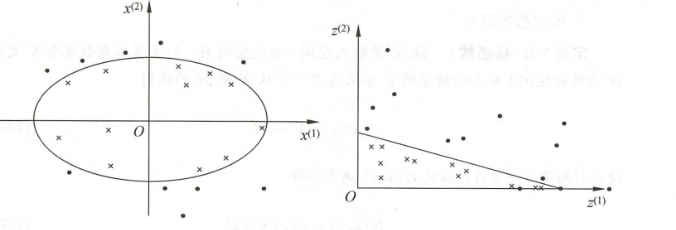
\includegraphics[scale=0.5]{figures/非线性分类问题和核技巧.png}
    \caption{非线性分类问题与核技巧}
    \label{非线性分类问题与核技巧}
\end{figure}

一般来说,对给定一个训练数据集$T=\{(x_1,y_1),(x_2,y_2),\cdots,(x_N,y_N)\}$,其中,实例
$x_i$属于输入空间,$x_i\in \mathbb{R}^n$,对应的标记有两类$y_i=\{-1,+1\}$,如果能用
$\mathbb{R}^n$中的一个\textsl{超曲面}将正负例正确分开,则称这个问题为\textsl{非线性可分问题}。

\subsection*{通过线性技巧解决非线性问题}
但是非线性问题往往不好求解,所以希望能用线性分类问题的方法去解决这类问题,所采取的方法是进行一个
\textsl{非线性变换},将非线性问题变成线性问题,通过解变换后的线性问题的方法求解原来的非线性问题。


\section{核函数的定义}
\begin{define}
    设$\mathcal{X}$是输入空间,$\mathcal{H}$为特征空间(希尔伯特空间),如果存在一个映射
    \begin{equation}
        \phi(\cdot):\mathcal{X}\rightarrow \mathcal{H}
    \end{equation}

    使得对于所有的$x,z\in \mathcal{X}$,函数$K(x,z)$满足条件
    \begin{equation}
        K(x,z)=\phi(x)\cdot \phi(z)
    \end{equation}

    则称$K(x,z)$为\textsl{\textbf{核函数}},$\phi(\cdot)$为映射函数。
\end{define}

核技巧的想法是,在学习与预测中只定义核函数$K(x,z)$,而不是显式地定义映射函数$\phi$。

\begin{example}
    假设假设输入空间是$\mathbb{R}^2$,核函数是$K(x,z)=(x\cdot z)^2$,找出相关特征空间$\mathcal{H}$和映射函数$\phi(x)$。
\end{example}

可以去特征空间为$\mathbb{R}^3$,记$x=(x^{(1)},x^{(2)})^T$,$z=(z^{(1)},z^{(2)})^T$
\begin{equation}
    (x\cdot z)^2=(x^{(1)}z^{(1)}+x^{(2)}z^{(2)})^2=(x^{(1)}z^{(1)})^2+2x^{(1)}z^{(1)}x^{(2)}z^{(2)}+(x^{(2)}z^{(2)})^2
\end{equation}

所以可以取映射
\begin{equation}
    \phi(x)=((x^{(1)})^2,\sqrt{2}x^{(1)}x^{(2)},(x^{(2)})^2)^T
\end{equation}

验证一下
\begin{equation}
    \phi(x)\cdot \phi(z)=(x\cdot z)^2=K(x,z)。
\end{equation}

仍然取$\mathcal{H}=\mathbb{R}^3$
\begin{equation}
    \phi(x)=\frac{1}{\sqrt{2}}((x^{(1)})^2-(x^{(2)})^2,
    2x^{(1)}x^{(2)},((x^{(1)})^2+(x^{(2)})^2)^T
\end{equation}

验证内积仍然得到核函数。

还可以取$\mathcal{H}=\mathbb{R}^4$
\begin{equation}
    \phi(x)=((x^{(1)})^2,(x^{(1)})(x^{(2)}),(x^{(1)})(x^{(2)}),(x^{(2)})^2)^2
\end{equation}

\section{核技巧在支持向量机中的应用}

在线性支持向量机的对偶问题中,无论是目标函数还是决策函数,都只涉及输入实例和实例直接的内积,在线性支持向量机的对偶问题的
目标函数中的内积$x_i\cdot x_j$可以用核函数$K(x_1,x_2)=\phi(x_i)\cdot \phi(x_j)$来替代。此时对偶问题的目标函数
\begin{equation}
    W(\alpha)=\frac{1}{2}\sum\limits_{i=1}^{N}\sum\limits_{j=1}^{N} \alpha_i\alpha_jy_iy_jK(x_i,x_j)-\sum\limits_{i=1}^{N}\alpha_i
\end{equation}

同样分类决策函数中的内积也可以用核函数来替代。
\begin{equation}
    f(x)=sign(\sum\limits_{i=1}^{N_s}\alpha^*_iy_iK(x_i,x)+b^*)
\end{equation}

这等价于经过映射函数将原来的输入空间变换到一个新的特征空间。在实际应用中,往往依赖领域知识直接选择核函数,
因此核函数的需要通过实验去验证。

\section{正定核}

不用构造映射$\phi(x)$能否直接判断一个给定的函数$K(x,z)$是不是核函数?

假设$K(x,z)\in \mathcal{X}\times \mathcal{X}$是对称函数,并且对任意的$x_1,x_2,\cdots,x_m\in \mathcal{X}$,$K(x,z)$
关于$x_1,x_2,\cdots,x_m$的Gram矩阵是半正定的。可以依据函数$K(x,z)$,构成一个希尔伯特空间,其步骤是,首先定义映射$\phi$并构成
向量空间$\mathcal{S}$,然后在$\mathcal{S}$上定义内积空间,最后讲$\mathcal{S}$完备化成希尔伯特空间。

\subsection*{定义映射,构成向量空间$\mathcal{S}$}

先定义映射
\begin{equation}
    \phi:x\rightarrow K(\cdot,x)
\end{equation}

根据这一映射,对任意$x_i\in \mathcal{X}$,$\alpha_i\in \mathbb{R}$,$i=1,2,\cdots,m$,定义线性组合
\begin{equation}
    f(\cdot)=\sum\limits_{i=1}^{m}\alpha_iK(\cdot,x_i)
\end{equation}


$\mathcal{S}$构成一个向量空间。

\subsection*{在$\mathcal{S}$上定义内积,使其成为内积空间}


在$\mathcal{S}$定义一个运算$*$,使得对于任意的$f,g\in\mathcal{S}$,

\begin{eqnarray}
    & f*g=\sum\limits_{i=1}^{m}\sum\limits_{j=1}^{l}\alpha_i\beta_jK(x_i,z_j)
\end{eqnarray}

其中
\begin{eqnarray}
    & f(\cdot)=\sum\limits_{i=1}^{m}\alpha_iK(\cdot,x_i)\\
    & g(\cdot)=\sum\limits_{j=1}^{l}\beta_iK(\cdot,z_i)
\end{eqnarray}

只需要验证$*$是$\mathcal{S}$上的内积

\begin{proposition}
    运算$*$是$\mathcal{S}$上的内积。\footnote{内积的性质:(1) 线性性;(2) 共轭对称;(3) 正定性}
\end{proposition}
\textbf{proof. }

\section{将内积空间$\mathcal{S}$完备化成希尔伯特空间}

定义内积的范数
\begin{equation}
    \Vert f\Vert=\sqrt{f\cdot f}
\end{equation}

则$\mathcal{S}$变成一个赋范线性空间,对于不完备的赋范线性空间$\mathcal{S}$,一定可以使之完备化,得到完备的
赋范线性空间$\mathcal{H}$。一个内积空间,当作为一个赋范空间是完备的时候,就是希尔伯特空间。

\subsection*{再生核希尔伯特空间}

这一希尔伯特空间$\mathcal{H}$称为\textsl{\textbf{再生核希尔伯特空间}(reproducing kernel Hilbert sapce,RKHS)},

这是由于核$K$的再生性。

\begin{define}
    (再生核)满足
    \begin{equation}
        K(\cdot,x)\cdot f=f(x)
    \end{equation}

    以及
    \begin{equation}
        K(\cdot,x)\cdot K(\cdot,z)=K(x,z)
    \end{equation}

    称为\textsl{\textbf{再生核}}
\end{define}

\subsection*{正定核的充要条件}
\begin{theorem}
    设$K:\mathcal{X}\times \mathcal{X}\rightarrow \mathbb{R}$是对称函数,则$K(x,z)$为正定核的充要条件是
    :对任意的$x_i\in \mathcal{X},i=1,2,\cdots,m$,$K(x,z)$对应的\textsl{Gram矩阵}
    \begin{equation}
        K=[K(x_i,x_j)]_{m\times m}
    \end{equation}

    是半正定矩阵。
\end{theorem}

\subsection*{正定核的等价定义}

\begin{define}
    设$\mathcal{X}\in \mathbb{R}^n$,$K(x,z)$是定义在$\mathcal{X}\times \mathcal{X}$上的对称函数,如果对任意的
    $x_i\in \mathcal{X},i=1,2,\cdots,m$,,$K(x,z)$对应的\textsl{Gram矩阵}
    \begin{equation}
        K=[K(x_i,x_j)]_{m\times m}
    \end{equation}

    是半正定矩阵,则$K(x,z)$是正定核。
\end{define}

这一定义在构造核函数的时候很有用,但是对于一个具体函数,检验他是核函数其实并不容易,在实际问题中往往应用已有的核函数。\textsl{Mercer定理}可以得到\textsl{Mercer核},
正定核比Mercer核更具有一般性。

\section{常用的核函数}

\subsection*{多项式核函数}

\begin{equation}
    K(x,z)=(x\cdot z+1)^p
\end{equation}

对应的支持向量机是一个$p$次多项式分类器。在此情形下,分类决策函数称为
\begin{equation}
    f(x)=sign(\sum\limits_{i=1}^{N_s}\alpha^*_iy_i(x_i\cdot x+1)^p+b^*)
\end{equation}

\subsection*{高斯核函数}

\begin{equation}
    K(x,z)=exp(-\frac{\Vert x-z\Vert^2}{2\sigma^2})
\end{equation}

对应的支持向量机是一个\textsl{\textbf{高斯径向基函数}(radial basis function)}。在此情形下,分类决策函数称为
\begin{equation}
    f(x)=sign(\sum\limits_{i=1}^{N_s}\alpha^*_iy_iexp(-\frac{\Vert x-z\Vert^2}{2\sigma^2})+b^*)
\end{equation}

\subsection*{字符串核函数}

字符串核是定义在字符串集合上的核函数,字符串核函数在文本分类,信息检索,生物信息学方面有所应用。

\section{非线性支持向量分类机算法}

\begin{define}
    从非线性分类训练集,通过核函数与软间隔最大化,或者凸二次规划学习到分类决策函数
    \begin{equation}
        f(x)=sign(\sum\limits_{i=1}^{N} \alpha^*_iy_iK(x,x_i)+b^*)
    \end{equation}

    称为非线性支持向量机,$K(x,z)$是正定核函数。
\end{define}

下面叙述非线性支持向量机学习算法

\subsection*{非线性支持向量机学习算法}
输入:训练数据集$T=\{(x_1,y_1),(x_2,y_2),\cdots,(x_N,y_N)\}$;
输出:分类决策函数
\begin{enumerate}[itemindent=2em]
    \item 选取适当核函数$K(x,z)$和适当的参数$C$,构造并求解最优化问题
    \begin{eqnarray}
        & \min\limits_{\alpha} \ \ &\frac{1}{2}\sum\limits_{i=1}^{N}\sum\limits_{j=1}^{N}
        \alpha_i\alpha_jy_iy_j(x_i\cdot x_j)K(x_i,x_j)-\sum\limits_{i=1}^{N}\alpha_i\\
        & s.t. & \sum\limits_{i=1}^{N}\alpha_iy_i=0\\
        &      & 0\leqslant \alpha_i\leqslant C,\ \ i=1,2,\cdots,N
    \end{eqnarray}

    求得最优解$\alpha^*$。
    \item 选择$\alpha^*$的一个正分量$0<\alpha^*_j<C$,计算
    \begin{equation}
        b^*=y_j-\sum\limits_{i=1}^{N}\alpha^*_iy_iK(x_i,x_j)
    \end{equation}
    \item 构造决策函数
    \begin{equation}
        f(x)=sign(\sum\limits_{i=1}^{N}\alpha^*_iy_iK(x,x_i)+b^*)
    \end{equation}

    当$K(x,z)$是正定核函数时,最优化问题时凸二次规划问题,解是存在的。
\end{enumerate}
